\documentclass{article}
\usepackage{amsmath}
\usepackage[a4paper, top=0.75in, bottom=0.75in]{geometry}
\usepackage{enumitem}
\usepackage{graphicx}

\graphicspath{ {./images/} }

\title{Homework 1}
\author{David Robinson}
\date{}
\setlength{\parindent}{0pt}

\begin{document}

\maketitle

\subsection*{Problem 1: Induction Review}

Base:
Let $n=1$. $\sum_{i=1}^1 i = 1$ and $\frac{1^2 + 1}{2} = \frac{1 + 1}{2} = \frac{2}{2} = 1$,
$LHS=RHS$ and the base case holds.
\vspace{1em}

Induction Hypothesis:
Accept $\sum_{i=1}^k i = \frac{k^2 + k}{2}$
\vspace{1em}

Induction:
Show $\sum_{i=1}^{k+1} i = \frac{{(k+1)}^2 + k + 1}{2}$

\[\begin{aligned}
    \sum_{i=1}^{k+1} i &= \sum_{i=1}^k i + k + 1 \quad & \text{summation} \\
    &= \frac{k^2 + k}{2} + k + 1 \quad & \text{induction hypothesis} \\
    &= \frac{k^2 + k}{2} + \frac{2 (k+1)}{2} \quad & \text{identity} \\
    &= \frac{k^2 + k}{2} + \frac{2k + 2}{2} \quad & \text{distribution} \\
    &= \frac{k^2 + k + 2k + 2}{2} \quad & \text{distribution} \\
    &= \frac{k^2 + 2k + 1 + k + 1}{2} \quad & \text{arithmetic} \\
    &= \frac{{(k+1)}^2 + k+1}{2} \quad & \text{arithmetic}
\end{aligned}\]

As desired, and we have shown the conclusion is true for all positive integers.

\subsection*{Problem 2: False Proofs Review}

When $k=1$, the induction hypothesis states that all horses are the same color.
\vspace{1em}

For $k+1=2$, we consider a set of two horses.
\begin{itemize}
    \item Removing the first horse leaves only the second horse in the set and by the induction hypothesis, all horses in the set are the same color.
    \item Removing the second horse leaves only the first horse in the set and by the induction hypothesis, all horses in the set are the same color.
\end{itemize}

While each subset satisfies the induction hypothesis, there is no guarantee that the first and second horse are the same color.

\subsection*{Problem 3: Graph Thinking}

In a graph with $n$ nodes and no self-loops, the degree of each node can range from $0$ (has no edges) to $n-1$ (is connected to every other node).
\vspace{1em}

However, a graph cannot have a node with a degree of $0$ and another with a degree of $n-1$, because if a node is connected to every other node, then every other node must have at least one edge, making it impossible for a node to have a degree of $0$. Therefore, while there are $n$ possible degree values, $[0, n-1]$, the graph can have at most $n-1$ distinct degrees values.
\vspace{1em}

Since there are $n$ nodes but only $n-1$ possible degree values, at least two nodes must have equal degrees.

\subsection*{Problem 4: DFA Construction}

\begin{enumerate}[label=\Alph*.]
    \item
    $q_0$: \textbf{Starting state or when there are an even number of a's and even number of b's, and the last character was `b'.} The string cannot start with `a' because then if `b' is added, it will contain the substring `ab' and there needs to be at least one `b' to have an odd number of `b's.
    
    $q_1$: \textbf{Accept state when there are an even number of a's and odd number of b's, and the last character was `a'.} The string cannot follow `a' with `b' or else the string will contain the substring `ab'.

    $q_2$: \textbf{Accept state when there are an even number of a's and odd number of b's, and the last character was `b'.}

    $q_3$: \textbf{When there are an odd number of a's and odd number of b's, and the last character was `a'.} The string cannot follow `a' with `b' or else the string will contain the substring `ab'.

    $q_4$: \textbf{Trap state when the string contains the substring `ab'.}
    
    \begin{center}
        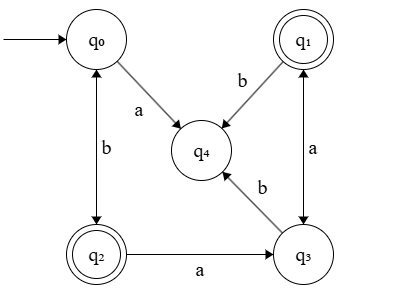
\includegraphics[scale=1]{dfa.png}
    \end{center}

    \item DFA that recognizes C
    
    \begin{center}
        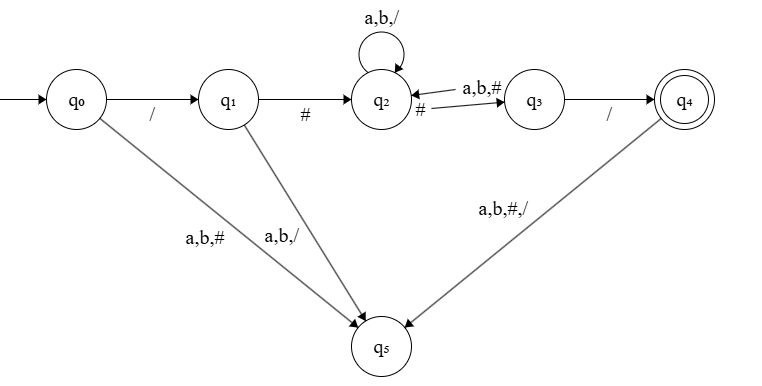
\includegraphics[scale=0.65]{dfa2.png}
    \end{center}
\end{enumerate}

\pagebreak

\subsection*{Problem 5: Regular Language Properties}

\begin{enumerate}[label=\Alph*.]
    \item You can obtain $\mathbf{M'}$ by swapping the accept and non-accept states in $M$, where all accept states are now non-accept states and all non-accept states are now accept staes.
    \item The complement of $\mathbf{B}$, contains all strings that are not in $\mathbf{B}$. By swapping the accept and non-accept states in $\mathbf{M}$, all strings that are accepted by $\mathbf{M}$ will be rejected by $\mathbf{M'}$ and all strings that are rejected by $\mathbf{M}$ will be accepted by $\mathbf{M'}$. Since a DFA separates strings into accepted and rejected groups, flipping these groups from $\mathbf{B}$ recognizes the complement of $\mathbf{B}$.
    \item Since all strings that are not accepted by a DFA recognizing a regular langauge $\mathbf{B}$ are accepted by a DFA recognizing its complement, the class of regular languages is closed under complement.
\end{enumerate}

\end{document}